\section{Introducción a OAI-PMH}\label{sec:oaipmh}

\acrfull{oaipmh} (actualmente disponible en su versión 2.0) es un protocolo para la transmisión de metadatos en Internet que surgió del esfuerzo de mejorar y abrir el acceso a archivos de publicaciones electrónicas (e-prints) y en general a un gran rango de materiales digitales que ha despertado el interés de la comunidad de bibliotecarios.\cite{JM_OAI}

\begin{figure}[!htp]
	\centering
	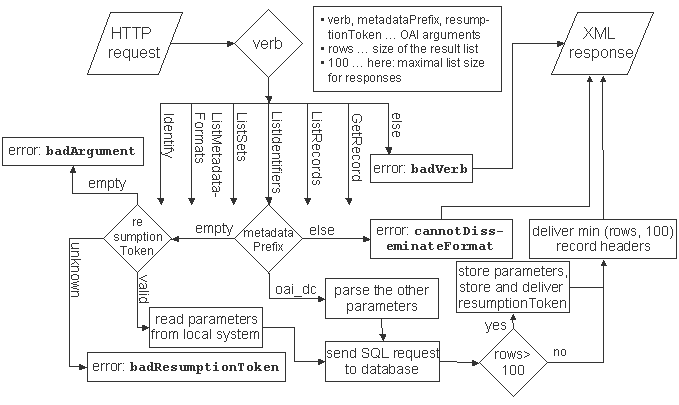
\includegraphics[scale=.15]{fig/oai_flow}
	\caption{Diagrama de flujo del servidor \acrshort{oaipmh}}\label{fig:oaiflow}
\end{figure}

El protocolo \acrshort{oaipmh} se basa en una arquitectura cliente-servidor en la que el cliente realiza las consultas por medio de transacciones \acrshort{http} GET o POST constituidas por un conjunto de opciones del tipo clave=valor. El servidor responde a la petición devolviendo un documento \acrshort{xml} bajo al menos el estandar \acrfull{dc}, según dicta la especificación de la implementación mínima del protocolo \acrshort{oaipmh} para los proveedores de información.\cite{OAIPMH_implementers}

Como se ve en la figura \ref{fig:oaiflow}\cite{oai_implementation} el cliente puede realizar seis peticiones al servidor en función del valor especificado en el `verb' de la consulta, las peticiones pueden ser:

\begin{itemize}
	\item \textbf{Idenfity:} Envía información sobre el servidor, así como el nombre del repositorio, \acrshort{url} base, correo electrónico del administrador del servidor, etc.
	\item \textbf{ListMetadataFormats:} Envía la lista de formatos en los que se encuentran disponibles los metadatos que al menos deben estar disponibles en \acrshort{dc}.
	\item \textbf{ListSets:} Envía una lista con los términos opcionales creados por el servidor para facilitar la recuperación selectiva de metadatos, posibilitando que un cliente pueda solicitar los registros pertenecientes a una clase en concreto. Estos términos representan una clasificación de los recursos según varias entradas. Los sets pueden estar compuestos por listas simple o formar una jerarquía.
	\item \textbf{ListIdentifiers: } Devuelve la cabecera de hasta un máximo de 100 registros por petición. Los identificadores pueden filtrarse por un rango entre dos fechas de creación o modificación o por los distintos ``sets'' definidos por el servidor.
	\item \textbf{ListRecords: } Realiza la misma tarea que la petición \textit{ListIdentifiers} a excepción de devolver el registro completo con sus metadatos, en lugar de incluir solo la cabecera del recurso. En caso de que la petición resulte una lista de más de 100 recursos, al igual que en la petición \textit{ListIdentifiers}, al final de la lista \acrshort{xml} se devolverá una clave `resumptionToken' que deberá ser utilizada por el cliente para continuar la devolución de los siguientes 100 registros en otra petición \acrshort{http} independiente.
	\item \textbf{GetRecord: } Petición utilizada para devolver un registro en concreto, siendo necesario especificar el identificador del recurso solicitado y el formato bibliográfico en el que se desea que se devuelva.
\end{itemize}

\clearpage

\lstinputlisting[language=XML, frame=single, label={lst:oaipmhgetrecord}, caption=Ejemplo de petición GetRecord de \acrshort{oaipmh}]{content/code/xml/get-record-example.xml}

El \acrshort{xml} generado por el servidor presenta la siguiente estructura para la extracción de los recursos:

\begin{itemize}
	\item \textbf{Información sobre la transacción:} El comienzo del \acrshort{xml} siempre está compuesto por atributos \textit{smlns}, \textit{smlns:xsi} y \textit{xsi:schemaLocation} que sirven para definir ``namespace'' y el esquema de \acrshort{oaipmh} del \acrshort{xml}.

	\item \textbf{La petición en cuestión:} En esta parte del \acrshort{xml} trata la información sobre una de las seis posibles peticiones. En el caso del GetRecords (véase algoritmo \ref{lst:oaipmhgetrecord}) por ejemplo, puede observarse que se compone de un elemento ``record'' y en el se subdivide en:
		\begin{itemize}
			\item Cabecera, en la que se especifica el identificador único, la fecha de creación o última modificación y la lista de ``sets'' a la que pertenece.
			\item Metadatos, la información misma del registro en cuestión compuesto por atributos tales como \textit{dc:title}, \textit{dc:creator}, \textit{dc:subjet}, y en general cualquiera de los atributos definidos en el set de elementos de \acrshort{dc}\cite{DCElements} o el formato bibliográfico que se haya especificado en la consulta.
		\end{itemize}
\end{itemize}